\section{Raw Gradients and Actual Updates under Adam}
\label{sec:adam-diagnostics}

The GD results distinguish local reversal from cumulative motion and objective
progress. Adam adds a second distinction: the raw gradient describes the current
loss slope, while the applied update depends on accumulated moments and coordinate
scaling. We use full-objective loss excursions to examine both quantities along
the same trajectory. This reveals whether a loss rise accompanies an update
that points uphill locally, or a finite step that rises despite pointing downhill.

\subsection{Loss-Slope Measurements along Adam Trajectories}

Adam~\cite{kingma2014adam} transforms the raw gradient through first-
and second-moment estimates,
\begin{equation}
\begin{aligned}
m_t&=\beta_1m_{t-1}+(1-\beta_1)g_t,\\
v_t&=\beta_2v_{t-1}+(1-\beta_2)g_t^{\odot2},
\end{aligned}
\label{eq:adam-moments}
\end{equation}
with zero initial moments. Bias correction gives
$\widehat m_t=m_t/(1-\beta_1^t)$ and
$\widehat v_t=v_t/(1-\beta_2^t)$, followed by
\begin{equation}
d_t=\frac{\widehat m_t}{\sqrt{\widehat v_t}+\epsilon},
\qquad \theta_t=\theta_{t-1}-\eta d_t,
\label{eq:adam-direction}
\end{equation}
where operations are coordinatewise and
$g_t=\nabla\mathcal L(\theta_{t-1})$ in the full-objective experiments.

Although $d_t$ determines the step, $g_t$ describes the local loss slope.
Changes in its direction and norm reveal how that slope varies across
the states visited by Adam. We retain $\rho_t$ for consecutive raw-gradient
cosine and denote the projected change by
\begin{equation}
\begin{aligned}
z_{t+1}
&:=1-\frac{g_t^\top g_{t+1}}{\|g_t\|^2}\\
&=1-\rho_{t+1}\frac{\|g_{t+1}\|}{\|g_t\|}.
\end{aligned}
\label{eq:adam-projected-response}
\end{equation}
This is the same numerical statistic denoted
$\eta\widehat\kappa_{t+1}$ in Eq.~\eqref{eq:kappa-estimate}.
For nonzero consecutive gradients, $z_{t+1}>1$ is equivalent to negative
alignment, while $z_{t+1}>2$ means
$g_t^\top g_{t+1}<-\|g_t\|^2$: the opposing projection exceeds the preceding
gradient's magnitude. These are geometric statements about the raw
gradients. The reference value two is not used as a universal loss-rise
threshold for Adam.

Consecutive first-moment cosines are labeled separately. They describe
the evolution of optimizer memory, while cross-alignment with the current
gradient, such as $\cos(g_t,\widehat m_t)$ or $\cos(g_t,d_t)$, answers
whether that memory and the actual update agree with the current slope.
We use both cross-alignments recorded at every optimizer boundary, and
the inner product of the raw gradient with the actual applied increment
to assess its first-order loss contribution.

\paragraph{Controlled trajectories.}

We reuse the CIFAR-10/MLP, CIFAR-10/ResNet-32 and WikiText-2/Transformer
objectives from Section~\ref{sec:gd-experiments}. Each Adam trajectory starts
from the same frozen, untrained seed-0 weights used for its GD comparison,
with fresh moments. We run 1,024 full-objective updates at each constant
rate: $\{0.0001,0.0003,0.001\}$ for the MLP and
$\{0.0003,0.001,0.003\}$ for ResNet and Transformer. All nine arms use
$(\beta_1,\beta_2)=(0.9,0.999)$ and $\epsilon=10^{-8}$, without a schedule,
clipping or weight decay. There is one initialization per model, matched
across rates. Full-batch accumulation removes sampling variation in the
objective; model, objective and numerical details are in
Appendix~\ref{appendix:adam-measurements}.

\begin{figure*}[tp]
 \centering
 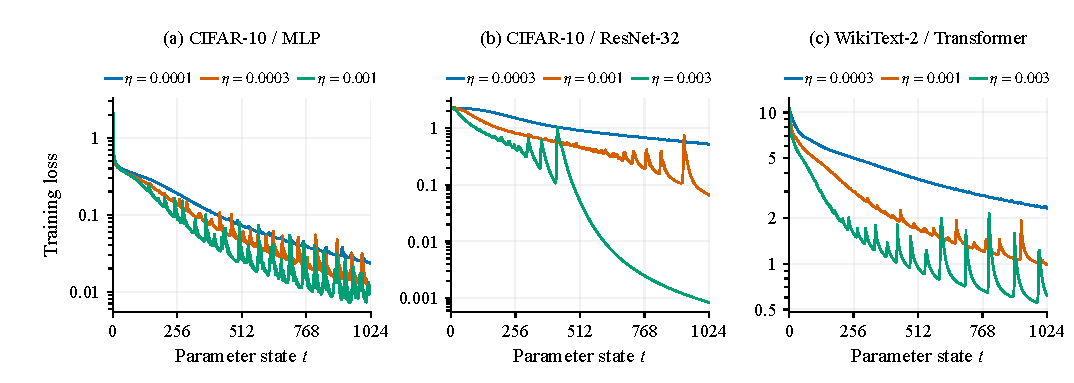
\includegraphics[width=\textwidth]{figures/analysis036/adam_manuscript_overview.pdf}
 \caption{Full-batch Adam training from matched initial weights, with three
 constant learning rates per model. Every training-loss observation is shown
 without smoothing on logarithmic y-axes. Horizontal axes count completed
 updates (labeled $t$ in the figure and denoted $s$ in the text). One initialization
 per model; colors identify increasing rates within each panel.}
 \label{fig:adam-overview}
\end{figure*}

Figure~\ref{fig:adam-overview} shows transient excursions within trajectories
whose longer-term training loss decreases. At 1,024 updates, the largest
tested rate attains the lowest final loss within each model's sweep.
We define the events using loss alone, then describe their population
statistics and individual temporal structure.

\subsection{Loss-Defined Events and Their Gradient Anatomy}

To examine repetition without selecting on gradients, write
$\mathcal L_s:=\mathcal L(\theta_s)$ for the recorded training loss.
Starting at initialization, let $a_i$ be the earliest available state with
$\mathcal L_{a_i+1}>\mathcal L_{a_i}$. Hold the pre-rise reference
$\mathcal L_{a_i}$ fixed. Recovery occurs at the first later state whose
loss is at or below this pre-rise level, $\mathcal L_s\leq\mathcal L_{a_i}$.
For an event recovered within $T$ updates, define
\begin{equation}
\begin{aligned}
 c_i&:=\min\{s:a_i<s\leq T,\ \mathcal L_s\leq\mathcal L_{a_i}\},\\
 p_i&\in\operatorname*{arg\,max}_{a_i<s<c_i}\mathcal L_s.
\end{aligned}
\label{eq:adam-spike-boundaries}
\end{equation}
If several states attain the maximum, $p_i$ is the earliest one.
Recovery summaries include only events recovered by $T=1024$;
incidence counts also retain right-censored events at that horizon.
Search resumes at $c_i$; partial declines and additional local maxima
before this return belong to the same event. Thus $a_i$ is the last
pre-rise state, $a_i+1$ the first elevated state, $p_i$ the loss peak,
and $c_i$ the first recovered state. Peak increase is
$100(\mathcal L_{p_i}/\mathcal L_{a_i}-1)$; rise and recovery times are
$p_i-a_i$ and $c_i-p_i$, in optimizer updates. The three loss ratios are
$1$, $\mathcal L_{p_i}/\mathcal L_{a_i}$ and
$\mathcal L_{c_i}/\mathcal L_{a_i}\leq1$.


The loss-only detector identifies 812 candidates: 806 recover by update 1,024
and six remain right-censored. We focus the anatomy comparison on the 129
recovered events with peak increase strictly greater than 10\%; two additional
above-threshold candidates are censored. The strict 5\% and 20\% cutoffs yield
206 and 74 recovered events, each with two censored candidates. The threshold
selects a population for description, rather than a dynamical boundary.
Table~\ref{tab:adam-incidence} gives counts and occupancy by trajectory.
Events within a trajectory are dependent, and the two larger-rate MLP arms
supply 84 of the 127 events with defined pre-rise cosine.

Pre-rise raw-gradient cosine is negative in 92.1\% of those 127 events.
At the loss peak, the raw-gradient norm exceeds its pre-rise value in every
one of the 129 recovered events. The mean and maximum relative peak increases
grow with rate in each model with more than one eligible rate, reaching a
maximum of 858.8\% for ResNet at $\eta=0.003$.
Mean recovery takes 17--19 updates versus 6--8 for the ResNet rise, and
24--31 versus about six for the Transformer; the MLP durations are more
comparable. These summaries describe the observed excursions, with separate
arrival-state and outgoing-step conventions specified in
Appendix~\ref{appendix:adam-measurements}.

\begin{table*}[tp]
 \caption{Anatomy of recovered spikes with peak increase greater than 10\%.
 Cells report mean $\pm$ sample SD across events; maximum peak increase has
 its own subcolumn. Before denotes a single diagnostic at state $a_i$;
 recovery denotes the event's mean over states $p_i+1,\ldots,c_i$.
 Norm ratios compare loss-peak/pre-rise and recovered/loss-peak endpoints.
 $N$ counts included events; dashes indicate no qualifying event.
 Two initialization events have undefined pre-rise diagnostics, leaving
 46 and 38 observations for those entries in the MLP's middle and highest
 LR rows. No smoothing or averaging across initializations.
 The raw $\eta\widehat\kappa$ columns report $z$ from
 Eq.~\eqref{eq:adam-projected-response}.}
 \label{tab:adam-spike-anatomy}
 \centering
 \footnotesize
 \setlength{\tabcolsep}{1.5pt}
 \renewcommand{\arraystretch}{1.15}
 % Generated by revisions/2026-11-03-regime-writing-revision/01_prepare_table.py.
\begin{tabular*}{\textwidth}{@{\extracolsep{\fill}}*{13}{c}@{}}
\toprule
\multirow{2}{*}{\shortstack{Dataset\\Model}} & \multirow{2}{*}{$\eta$} & \multirow{2}{*}{$N$} & \multicolumn{2}{c}{Peak increase (\%)} & \multicolumn{2}{c}{Time (updates)} & \multicolumn{2}{c}{$\eta\widehat\kappa$ (raw)} & \multicolumn{2}{c}{$\rho$ (raw)} & \multicolumn{2}{c}{Gradient norm ratio} \\
\cmidrule(lr){4-5}\cmidrule(lr){6-7}\cmidrule(lr){8-9}\cmidrule(lr){10-11}\cmidrule(lr){12-13}
 & & & Mean $\pm$ SD & Max & Rise & Recovery & Before & Recovery & Before & Recovery & Rise & Recovery \\
\midrule
\multirow{3}{*}{\shortstack{CIFAR-10\\MLP}} & $10^{-4}$ & 8 & $19\,\mathord{\pm}\,6.1$ & 31 & $8.4\,\mathord{\pm}\,2.9$ & $4.4\,\mathord{\pm}\,2.4$ & $1.8\,\mathord{\pm}\,0.38$ & $1.7\,\mathord{\pm}\,0.08$ & $-0.77\,\mathord{\pm}\,0.31$ & $-0.89\,\mathord{\pm}\,0.08$ & $5.3\,\mathord{\pm}\,1.7$ & $0.30\,\mathord{\pm}\,0.07$ \\
 & $3\times10^{-4}$ & 47 & $43\,\mathord{\pm}\,46$ & 203 & $5.5\,\mathord{\pm}\,4.4$ & $4.9\,\mathord{\pm}\,4.0$ & $1.3\,\mathord{\pm}\,0.25$ & $1.6\,\mathord{\pm}\,0.18$ & $-0.53\,\mathord{\pm}\,0.29$ & $-0.71\,\mathord{\pm}\,0.24$ & $4.5\,\mathord{\pm}\,3.0$ & $0.33\,\mathord{\pm}\,0.13$ \\
 & $10^{-3}$ & 39 & $95\,\mathord{\pm}\,107$ & 318 & $6.1\,\mathord{\pm}\,5.9$ & $7.4\,\mathord{\pm}\,7.5$ & $1.4\,\mathord{\pm}\,0.40$ & $1.4\,\mathord{\pm}\,0.26$ & $-0.46\,\mathord{\pm}\,0.38$ & $-0.55\,\mathord{\pm}\,0.30$ & $5.2\,\mathord{\pm}\,3.8$ & $0.31\,\mathord{\pm}\,0.14$ \\
\midrule
\multirow{3}{*}{\shortstack{CIFAR-10\\ResNet-32}} & $3\times10^{-4}$ & 0 & -- & -- & -- & -- & -- & -- & -- & -- & -- & -- \\
 & $10^{-3}$ & 10 & $105\,\mathord{\pm}\,182$ & 602 & $7.5\,\mathord{\pm}\,2.2$ & $17\,\mathord{\pm}\,11$ & $1.3\,\mathord{\pm}\,0.39$ & $1.3\,\mathord{\pm}\,0.25$ & $-0.36\,\mathord{\pm}\,0.42$ & $-0.36\,\mathord{\pm}\,0.26$ & $4.3\,\mathord{\pm}\,2.9$ & $0.43\,\mathord{\pm}\,0.24$ \\
 & $3\times10^{-3}$ & 7 & $179\,\mathord{\pm}\,309$ & 859 & $6.3\,\mathord{\pm}\,1.3$ & $19\,\mathord{\pm}\,20$ & $1.7\,\mathord{\pm}\,0.38$ & $1.1\,\mathord{\pm}\,0.37$ & $-0.65\,\mathord{\pm}\,0.28$ & $-0.13\,\mathord{\pm}\,0.42$ & $5.0\,\mathord{\pm}\,4.2$ & $0.34\,\mathord{\pm}\,0.24$ \\
\midrule
\multirow{3}{*}{\shortstack{WikiText-2\\Transformer}} & $3\times10^{-4}$ & 0 & -- & -- & -- & -- & -- & -- & -- & -- & -- & -- \\
 & $10^{-3}$ & 6 & $33\,\mathord{\pm}\,25$ & 81 & $6.3\,\mathord{\pm}\,1.9$ & $24\,\mathord{\pm}\,9.8$ & $2.1\,\mathord{\pm}\,0.27$ & $0.96\,\mathord{\pm}\,0.16$ & $-0.84\,\mathord{\pm}\,0.10$ & $-0.02\,\mathord{\pm}\,0.12$ & $9.0\,\mathord{\pm}\,3.8$ & $0.09\,\mathord{\pm}\,0.05$ \\
 & $3\times10^{-3}$ & 12 & $82\,\mathord{\pm}\,70$ & 231 & $6.2\,\mathord{\pm}\,2.7$ & $31\,\mathord{\pm}\,17$ & $2.2\,\mathord{\pm}\,0.43$ & $0.91\,\mathord{\pm}\,0.19$ & $-0.79\,\mathord{\pm}\,0.22$ & $0.09\,\mathord{\pm}\,0.21$ & $11\,\mathord{\pm}\,6.9$ & $0.08\,\mathord{\pm}\,0.08$ \\
\bottomrule
\end{tabular*}

\end{table*}

In Table~\ref{tab:adam-spike-anatomy}, diagnostics at parameter state $s$
use gradient index $s+1$. Recovery first averages within each event, then
weights events equally. Norm ratios compare the pre-rise, peak and recovered
endpoints; the gradient norm's maximum need not coincide with the loss peak.

\paragraph{Individual trajectories.}
For each model, we illustrate the recovered excursion with the largest
peak/pre-rise loss ratio at its highest tested rate. Selection uses
loss alone, with no condition on a gradient diagnostic. The peaks occur
at states 703, 422, and 794 for the MLP, ResNet, and Transformer.

\begin{figure*}[tp]
 \centering
 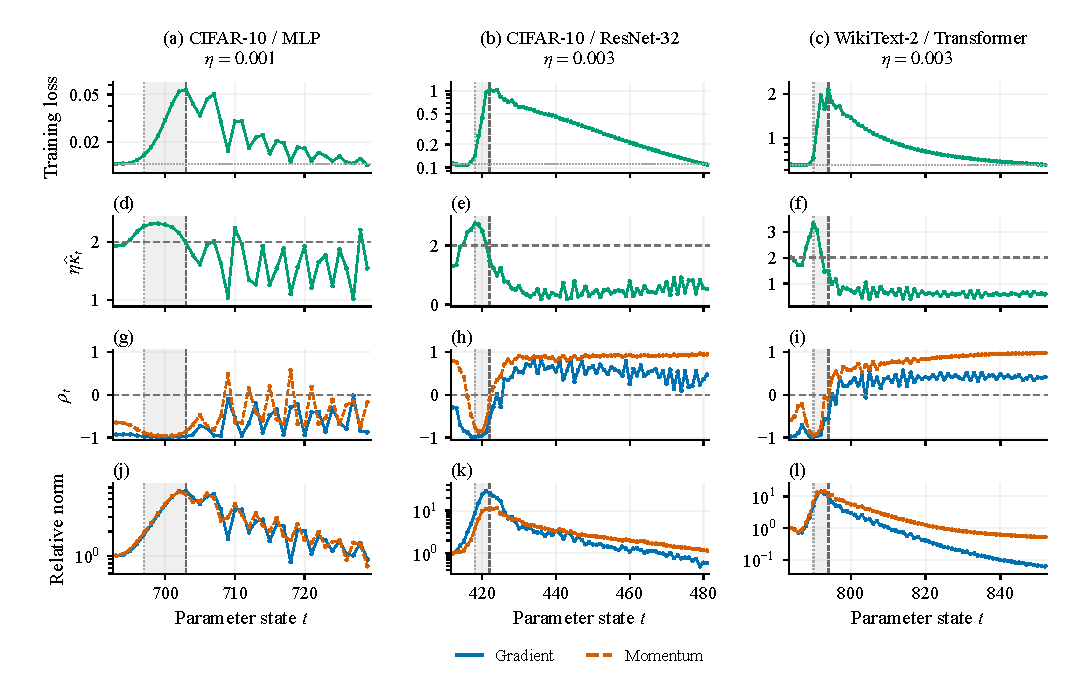
\includegraphics[width=\textwidth]{figures/analysis036/adam_manuscript_spikes.pdf}
 \caption{Largest recovered relative loss spike at each model's highest
 Adam rate. Rows show loss, raw-gradient projected change, consecutive
 cosines of raw gradients and first moments, and their relative norms.
 All observations are unsmoothed. The horizontal state count is labeled $t$;
 at state $s$ in the text, diagnostics refer to $g_{s+1}$ and $m_{s+1}$. Norms are divided by their value at the
 first displayed state. Gray bands mark the pronounced rise from the first
 +10\% crossing to the loss peak (697--703, 418--422 and 790--794), rather
 than the entire excursion through recovery. The horizontal dotted loss
 reference is the first displayed loss. Windows begin ten states before
 the peak and end at the first later loss below that displayed reference.}
 \label{fig:adam-spikes}
\end{figure*}

All three examples in Fig.~\ref{fig:adam-spikes} enter the pronounced rise
with negative raw-gradient cosine. During the rise, raw-gradient norms
increase sharply, the projected response exceeds two before the loss
maximum, and first-moment norms grow.

Recovery distinguishes the examples. ResNet and Transformer return to
positive raw-gradient and consecutive first-moment alignment, with a
falling projected response and a comparatively smooth loss decline.
The MLP continues to oscillate: its raw-gradient cosine remains mostly
negative, first-moment cosine alternates, and loss and norms decrease
through repeated rebounds. Thus, the illustrations share reversal and
amplification during the rise while exhibiting different recovery
patterns. Population-level phase comparisons are needed to determine
how consistently these patterns recur across initializations.

\subsection{Finite-Step Loss Rise with a Descending Local Direction}

Across all 129 recovered events, every one of the 794 outgoing steps
from $a_i$ through $p_i-1$ has
$g_{s+1}^{\top}(\theta_{s+1}-\theta_s)<0$. Thus each rise interval
consists of locally descending steps, although the loss increases
overall. During recovery, 1,374 of 1,376 outgoing steps have the same
negative first-order contribution. Event-mean
$\cos(g_t,d_t)$ during rise ranges from 0.071 to 0.767 across the
seven eligible trajectories. Negative consecutive raw-gradient cosine
therefore need not mean that Adam moves against the current local
descent direction. First-order descent alone also does not ensure
a decrease over the finite applied step.

For a smooth objective and actual increment
$u_t=\theta_t-\theta_{t-1}$, the exact loss change separates into
\begin{equation}
\begin{aligned}
\mathcal L(\theta_t)-\mathcal L(\theta_{t-1})
={}&g_t^\top u_t\\
&+\int_0^1(1-s)u_t^\top
H(\theta_{t-1}+su_t)u_t\,ds.
\end{aligned}
\label{eq:actual-step-loss}
\end{equation}
The negative linear contribution measures a descending tangent, while the
remaining term accounts for variation along the finite step. The measured
net rise requires the summed finite-step remainder to outweigh the descending
linear contributions. This observation rules out an explanation based solely
on Adam pointing uphill at those states; it does not isolate which aspect of
optimizer memory or coordinate scaling produced the finite-step behavior.
For nonsmooth objectives, the measured loss-minus-linear residual remains
defined even when this classical-Hessian integral is not applicable.

\subsection{What Reversal Does and Does Not Diagnose}

Ordinary oscillatory training provides a reference for the event summaries.
In the lowest-rate ResNet and Transformer arms, 726/953 and 764/953 eligible
states have negative raw cosine, respectively, and 186/953 and 215/953 have
$z>2$. None is followed by a loss rise of at least 10\% within eight updates.
Eligibility requires state $s\ge64$, a complete eight-update future and
current loss less than 5\% above the trailing 16-state minimum.
These fixed-horizon controls establish that both signatures occur during
ordinary training. They are not duration-matched comparisons to the
recovered events.

Norm amplification also explains much of the variation in event severity.
In a retained comparison on the same 127 events, adding pre-rise cosine to
log norm amplification improves within-trajectory fits but increases
held-out squared error in all seven eligible leave-one-rate-out comparisons.
Appendix~\ref{appendix:adam-measurements} specifies those retrospective fits.
Thus the anatomy establishes recurring gradient behavior without supporting
a transferable severity rule based on alignment.

The raw response remains useful as a description of the traversed loss
landscape. For smooth full-batch Adam,
$g_{t+1}-g_t=-\eta\overline H_t d_t$, where $\overline H_t$ averages the
Hessian along the update. Consequently,
$z_{t+1}/\eta=g_t^\top\overline H_t d_t/\|g_t\|^2$ is a mixed projection
involving the gradient and the applied direction, rather than the GD
Rayleigh quotient. Appendix~\ref{appendix:adam-memory} relates it to the
one-HVP proxy of Bai et al.~\cite{bai2026adaptive}, separating first-moment
and finite-step corrections. Agreement with that proxy has not been measured
here. The empirical conclusion is instead direct: raw-gradient reversal,
optimizer direction and finite-step objective change must be read separately.
